%--------------------------------------------------------
\section{Deployment} \label{sec:deployment}
%--------------------------------------------------------

Without an equally minimalist build process, creating Coexist would not be
productive. The two likely users of Coexist are programmers and IT specialists.
For programmers that work with Android every day, designing and building a
simple data access application may not be difficult. Coexist must be obviously
more simple than building an Android application if programmers are going
to consider using it. Likewise, a simple build process will allow IT specialists
to build and configure Coexist without needing to learn a programming language.

Section~\ref{sec:api} introduced the problems that Coexist needed to solve in
order to be an effective data access system. Section~\ref{sec:replication}
specified the method and protocol that clients use to synchronize themselves
with the server. Section~\ref{sec:metamodel} tied everything together by
creating a metamodel of all information that clients need to display and collect
data to and from users. In this section, we explain what users have to do in
order to use Coexist, starting with Figure~\ref{fig:coexist_project}.



\usetikzlibrary{trees}
\begin{figure}[h!]
\centering
\begin{tikzpicture}[scale=.7, every node/.style={transform shape},%
  grow via three points={one child at (0.5,-0.7) and
  two children at (0.5,-0.7) and (0.5,-1.4)},
  edge from parent path={(\tikzparentnode.south) |- (\tikzchildnode.west)}]
  \node [dir]  {myproject}
    child {node [dir] {ui}
      child {node [dir] {1}
        child {node [file] {metamodel.json}}
      }
    }
    child [missing] {}
    child [missing] {}
    child {node [file] {coexist.ini}}
    child {node [file] {logo.png}}
    child {node [file] {notification.png}}

    ;
\end{tikzpicture}
\caption{File structure for a Coexist project, where dashed lines are folders.
Users only specify the information that is unique to their application and the
\var{coexist} executable will create and compile the necessary code.}
\label{fig:coexist_project}
\end{figure}


Figure~\ref{fig:coexist_project} depicts the file structure of a Coexist project
directory: all information that is unique to any given application. The
\var{logo.png} and \var{notification.png} are 72x72 pixel icons that the
application uses for launchers and notifications, respectively. The \var{ui}
directory contains any number of directories with integer names. The integer
name corresponds to the current version of Coexist, as defined in the
\var{coexist.ini} file. Each of these integer based directories contains a JSON
metamodel described in Section~\ref{sec:metamodel}. In this case, the
application has defined a metamodel for version 1. Having this file structure
allows users to easily roll back to a prior version by changing the version
number in \var{coexist.ini}. 

The \var{coexist.ini} file is the aggregate of most of the unique information to
the application. This includes server URL location, deployment options, client
specific features and more. The following section will explain all of the
options that \var{coexist.ini} offers users. 


%--------------------------------------------------------
\subsection{coexist.ini file}  \label{sec:ini}

The purpose of the \var{coexist.ini} file is to give users a single space to
enumerate all of the information that Coexist needs to know about an
application. 

% use relative file paths

\begin{enumerate}
    \setlength{\parskip}{0cm}%
\item \bt{name} The name of the application. It will be seen in the main window
  of the Android application, title of Web pages etc.

\item \bt{image} An image icon for the application. On Android, this will be the
  icon that users click to launch the application.

\item \bt{notification} An image icon for the application's notifications. This
  can optionally be the same as the \texttt{image} parameter, but most Android
  applications have a grey scale version of \texttt{image} here instead.

\item \bt{package} The unique java style domain for your application. If a
  particular instance is going to be an inventory application for a company with
  the domain \texttt{domain.com} then this field might be \texttt{com.domain.inventory}.
  This field is important because Android requires all applications to have a
  unique package name. 

\item \bt{api} The URL of the Coexist server API. If this is the first time
  Coexist is being configured then the server API would not have been deployed
  yet, but the location is still required. This field could be
  \texttt{http://domain.com/api/}; this is the URL that the clients will send their
  requests to. 

\item \bt{version} This is the current version of the application (i.e. 1). This
  will ultimately reside in a directory of the server API (that gets created
  using this file) \texttt{conf/conf.ini}. If it is ever incremented then it will
  reject all client requests that are using different versions with a 409 error
  code and cause them to resync and upgrade. More on this in the server section
  ??.

\item \bt{user} The user name of the database for the server API's use.

\item \bt{pass} The password of the database for the server API's use.

\item \bt{db} The name of the database for the server API's use.

\item \bt{host} The hostname of the database for the server API's use.

\item \bt{dbms} The database type (i.e. mysql, postgresql) for use in the server
  API's PHP PDO calls. It should support any database type that the PDO library
  does.

\item \bt{ui} The location of the ui dir that should be included in the server
  API. This is the relative file path to the ui dir depicted in
  Figure~\ref{fig:coexist_project}
%\item \bt{sql} The location of the sql dir that should be included in the
%server API. This is explained further in the SQL Dir section ??.

\item \bt{android} An on/off value can be used to enable or disable the Android
  build. If the Android client is going to be built, then the user must have the
  Android SDK installed and the \var{android} and \var{adb} binaries should be on
  the path.

\item \bt{web} An on/off value can be used to enable or disable the server API
  build.

\item \bt{scp\_to} An experimental key that can be used to better automate the
  build process. A possible value might be
  \texttt{user@domain.com:/srv/domain.com/}. This would cause the resulting apk and
  tgz packages to be copied to the target server using scp. The public facing
  content in the tgz package is in a folder named htdocs, so the sample
  \texttt{scp\_to} value would be especially wise if the document root was
  \texttt{/srv/domain.com/htdocs} because a simple un-tar would be all that was
  required. 

\item \bt{scp\_port} Just in case the ssh server is running on a non standard
  port.

\end{enumerate}

When all of this information has be added, the \var{coexist} executable can be
used to create an instance of the application.

%--------------------------------------------------------
\subsection{coexist executable}  \label{sec:exe}

% each client code in separate repository
% exe will call ./configure on each client, passing info from ini

Assuming a file structure like the one in Figure~\ref{fig:coexist_project}, and
a filled out \var{coexist.ini}, users can use the \var{coexist} executable to
create installable packages for the server and clients. In Coexist, all client
projects have a configure script and are stored in separate repositories. The
\var{coexist} executable, which is a small bash script, will parse the
\var{coexist.ini} file, download the appropriate client code, pass relevant
entries from \var{coexist.ini} to client's configure scripts and build them.
All of resulting packages will be placed into a ``bin'' directory within the
project. If the \var{scp\_to} field is filled out in \var{coexist.ini}, then the
server side code will be copied over to the server using \var{scp}, where it can
be decompressed and ready to use.






%--------------------------------------------------------
\subsection{Use the client!}  \label{sec:}

At this point, the Coexist system is fully functional and any client that
installs the appropriate package can interface with the server. This section uses the
Android client as an example.


\begin{figure}[h!]
    \centering
    \begin{subfigure}[b]{0.25\textwidth}
        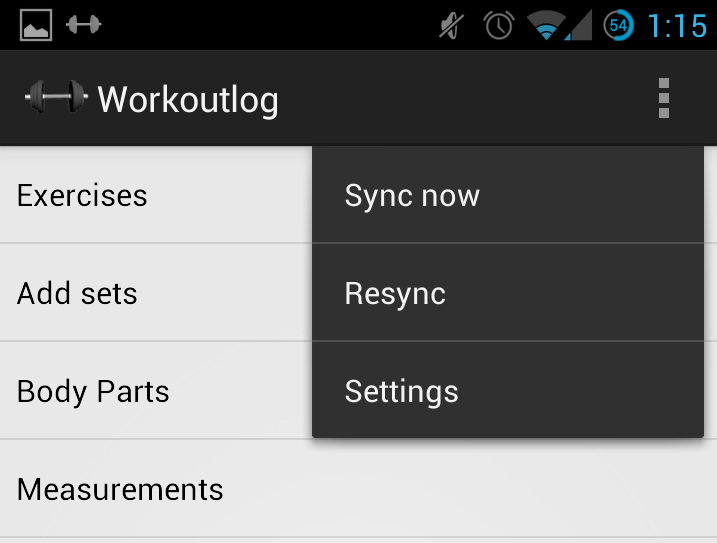
\includegraphics[width=.9\textwidth]{images/ss/menu.png}
        \label{fig:gull}
    \end{subfigure}%
    \begin{subfigure}[b]{0.25\textwidth}
        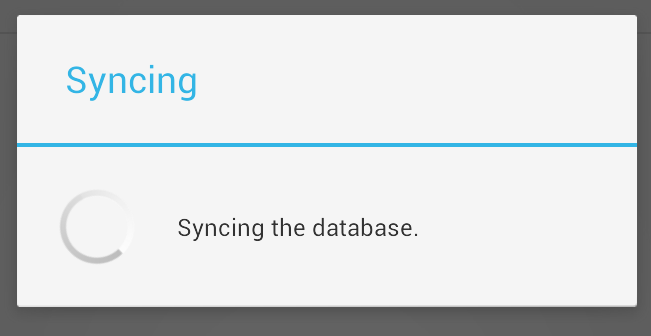
\includegraphics[width=.9\textwidth]{images/ss/syncing.png}
        \label{fig:tiger}
    \end{subfigure}
    \caption{This is the home screen of the Coexist Android client after its
    first launch and sync. The screen contains a list of items that correspond
  to database tables.}
    \label{fig:start_screen}
\end{figure}


On first luanch, the client will start its initial synchronization, where it will go
through the states described in Figure~\ref{fig:client_states} in
Section~\ref{sec:api}. In short, the client will download the metamodel and
schema from the server, then make a sync request to \sync as described in
Section~\ref{sec:replication}. The contents of the home screen are decided by
the JSON metamodel. Every \var{form} object in the metamodel will map to an
entry on the home screen. Clicking on any of the home screen items will bring up
an appropriate form screen for browsing and adding data.
Figure~\ref{fig:add_screen} contains the ``add'' portion of the form screen for
the ``Add sets'' home screen item. 


\begin{figure}[h!]
    \centering
    \begin{subfigure}[3a]{0.25\textwidth}
        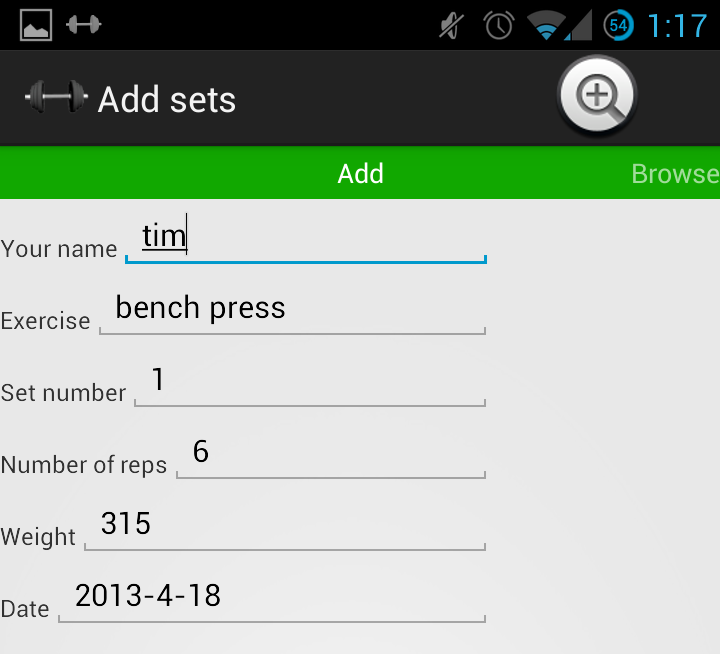
\includegraphics[width=.9\textwidth]{images/ss/form.png}
        \label{fig:gull}
    \end{subfigure}%
    \begin{subfigure}[3a]{0.25\textwidth}
        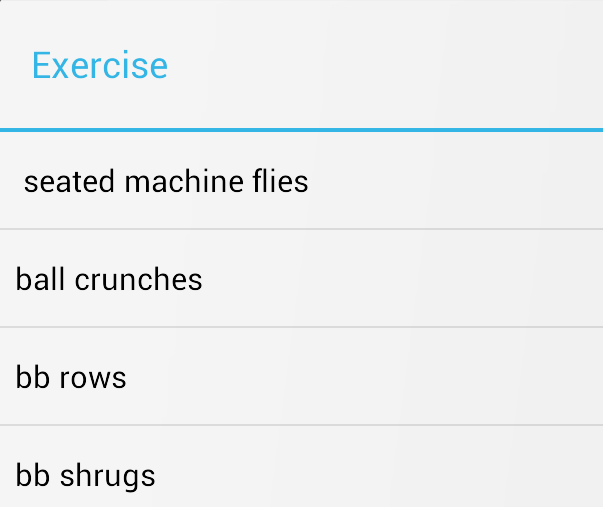
\includegraphics[width=.9\textwidth]{images/ss/fk.png}
        \label{fig:tiger}
    \end{subfigure}
    \caption{The add form for the \var{Exercise} table of a Coexist instance.
    The \var{Exercise} field corresponds to a column that references some other
    column. The menu on the right is an enumeration of the valid values that
  users can select from.}
    \label{fig:add_screen}
\end{figure}

Every field on the form screen has a type, as explained in
Section~\ref{sec:types}. In this case, the \var{Your name} field is a string,
\var{Set number}, \var{number of reps}, and \var{weight} are integers,
\var{Date} is a date and \var{Exercise} is a reference. Recall that the type
system is used for input filtering. The ``Exercises'' list in
Figure~\ref{fig:add_screen} is what appears when attempting to set the
\var{Exercise} field. Similarly, a date picker is launched for entering date
values and the integer fields don't accept non-integer input at all.

%Once the application is installed and opened, the screen will be blank and spinning. 
%
%\begin{figure}[h!]
%\centering
%
\includegraphics[width=0.25\textwidth]{images/new.png}
%\caption{ShoppingList on first launch.}
%\label{fig:first_launch}
%\end{figure}
%
%In the overflow menu there is an option called \texttt{Sync Now} that will trigger a sync.
%
%\begin{figure}[h!]
%\centering
%
\includegraphics[width=0.25\textwidth]{images/dl.png}
%\caption{ShoppingList after first sync.}
%\label{fig:first_sync}
%\end{figure}
%
%This will cause the client to request the appropriate SQL file and JSON meta
%model file from the server. Using this, it will create a local version of the
%database and request all missing rows (which will be all rows). It will finish
%by reporting the total amount of rows that it received, as seen in
%Figure~\ref{fig:first_sync}



%At this point the application is fully functional. Clicking on the
%\texttt{Items} section in the home screen will bring launch the CRUD screen for
%it. Swiping to the right will reveal the UI form generated by the JSON meta
%model and swiping to the left will allow browsing of the database contents. 




